% Options for packages loaded elsewhere
\PassOptionsToPackage{unicode}{hyperref}
\PassOptionsToPackage{hyphens}{url}
%
\documentclass[
]{book}
\usepackage{amsmath,amssymb}
\usepackage{lmodern}
\usepackage{iftex}
\ifPDFTeX
  \usepackage[T1]{fontenc}
  \usepackage[utf8]{inputenc}
  \usepackage{textcomp} % provide euro and other symbols
\else % if luatex or xetex
  \usepackage{unicode-math}
  \defaultfontfeatures{Scale=MatchLowercase}
  \defaultfontfeatures[\rmfamily]{Ligatures=TeX,Scale=1}
\fi
% Use upquote if available, for straight quotes in verbatim environments
\IfFileExists{upquote.sty}{\usepackage{upquote}}{}
\IfFileExists{microtype.sty}{% use microtype if available
  \usepackage[]{microtype}
  \UseMicrotypeSet[protrusion]{basicmath} % disable protrusion for tt fonts
}{}
\makeatletter
\@ifundefined{KOMAClassName}{% if non-KOMA class
  \IfFileExists{parskip.sty}{%
    \usepackage{parskip}
  }{% else
    \setlength{\parindent}{0pt}
    \setlength{\parskip}{6pt plus 2pt minus 1pt}}
}{% if KOMA class
  \KOMAoptions{parskip=half}}
\makeatother
\usepackage{xcolor}
\IfFileExists{xurl.sty}{\usepackage{xurl}}{} % add URL line breaks if available
\IfFileExists{bookmark.sty}{\usepackage{bookmark}}{\usepackage{hyperref}}
\hypersetup{
  pdftitle={BIOSCI 0835 Our Changing World Syllabus},
  pdfauthor={Nathan L. Brouwer},
  hidelinks,
  pdfcreator={LaTeX via pandoc}}
\urlstyle{same} % disable monospaced font for URLs
\usepackage{color}
\usepackage{fancyvrb}
\newcommand{\VerbBar}{|}
\newcommand{\VERB}{\Verb[commandchars=\\\{\}]}
\DefineVerbatimEnvironment{Highlighting}{Verbatim}{commandchars=\\\{\}}
% Add ',fontsize=\small' for more characters per line
\usepackage{framed}
\definecolor{shadecolor}{RGB}{248,248,248}
\newenvironment{Shaded}{\begin{snugshade}}{\end{snugshade}}
\newcommand{\AlertTok}[1]{\textcolor[rgb]{0.94,0.16,0.16}{#1}}
\newcommand{\AnnotationTok}[1]{\textcolor[rgb]{0.56,0.35,0.01}{\textbf{\textit{#1}}}}
\newcommand{\AttributeTok}[1]{\textcolor[rgb]{0.77,0.63,0.00}{#1}}
\newcommand{\BaseNTok}[1]{\textcolor[rgb]{0.00,0.00,0.81}{#1}}
\newcommand{\BuiltInTok}[1]{#1}
\newcommand{\CharTok}[1]{\textcolor[rgb]{0.31,0.60,0.02}{#1}}
\newcommand{\CommentTok}[1]{\textcolor[rgb]{0.56,0.35,0.01}{\textit{#1}}}
\newcommand{\CommentVarTok}[1]{\textcolor[rgb]{0.56,0.35,0.01}{\textbf{\textit{#1}}}}
\newcommand{\ConstantTok}[1]{\textcolor[rgb]{0.00,0.00,0.00}{#1}}
\newcommand{\ControlFlowTok}[1]{\textcolor[rgb]{0.13,0.29,0.53}{\textbf{#1}}}
\newcommand{\DataTypeTok}[1]{\textcolor[rgb]{0.13,0.29,0.53}{#1}}
\newcommand{\DecValTok}[1]{\textcolor[rgb]{0.00,0.00,0.81}{#1}}
\newcommand{\DocumentationTok}[1]{\textcolor[rgb]{0.56,0.35,0.01}{\textbf{\textit{#1}}}}
\newcommand{\ErrorTok}[1]{\textcolor[rgb]{0.64,0.00,0.00}{\textbf{#1}}}
\newcommand{\ExtensionTok}[1]{#1}
\newcommand{\FloatTok}[1]{\textcolor[rgb]{0.00,0.00,0.81}{#1}}
\newcommand{\FunctionTok}[1]{\textcolor[rgb]{0.00,0.00,0.00}{#1}}
\newcommand{\ImportTok}[1]{#1}
\newcommand{\InformationTok}[1]{\textcolor[rgb]{0.56,0.35,0.01}{\textbf{\textit{#1}}}}
\newcommand{\KeywordTok}[1]{\textcolor[rgb]{0.13,0.29,0.53}{\textbf{#1}}}
\newcommand{\NormalTok}[1]{#1}
\newcommand{\OperatorTok}[1]{\textcolor[rgb]{0.81,0.36,0.00}{\textbf{#1}}}
\newcommand{\OtherTok}[1]{\textcolor[rgb]{0.56,0.35,0.01}{#1}}
\newcommand{\PreprocessorTok}[1]{\textcolor[rgb]{0.56,0.35,0.01}{\textit{#1}}}
\newcommand{\RegionMarkerTok}[1]{#1}
\newcommand{\SpecialCharTok}[1]{\textcolor[rgb]{0.00,0.00,0.00}{#1}}
\newcommand{\SpecialStringTok}[1]{\textcolor[rgb]{0.31,0.60,0.02}{#1}}
\newcommand{\StringTok}[1]{\textcolor[rgb]{0.31,0.60,0.02}{#1}}
\newcommand{\VariableTok}[1]{\textcolor[rgb]{0.00,0.00,0.00}{#1}}
\newcommand{\VerbatimStringTok}[1]{\textcolor[rgb]{0.31,0.60,0.02}{#1}}
\newcommand{\WarningTok}[1]{\textcolor[rgb]{0.56,0.35,0.01}{\textbf{\textit{#1}}}}
\usepackage{longtable,booktabs,array}
\usepackage{calc} % for calculating minipage widths
% Correct order of tables after \paragraph or \subparagraph
\usepackage{etoolbox}
\makeatletter
\patchcmd\longtable{\par}{\if@noskipsec\mbox{}\fi\par}{}{}
\makeatother
% Allow footnotes in longtable head/foot
\IfFileExists{footnotehyper.sty}{\usepackage{footnotehyper}}{\usepackage{footnote}}
\makesavenoteenv{longtable}
\usepackage{graphicx}
\makeatletter
\def\maxwidth{\ifdim\Gin@nat@width>\linewidth\linewidth\else\Gin@nat@width\fi}
\def\maxheight{\ifdim\Gin@nat@height>\textheight\textheight\else\Gin@nat@height\fi}
\makeatother
% Scale images if necessary, so that they will not overflow the page
% margins by default, and it is still possible to overwrite the defaults
% using explicit options in \includegraphics[width, height, ...]{}
\setkeys{Gin}{width=\maxwidth,height=\maxheight,keepaspectratio}
% Set default figure placement to htbp
\makeatletter
\def\fps@figure{htbp}
\makeatother
\setlength{\emergencystretch}{3em} % prevent overfull lines
\providecommand{\tightlist}{%
  \setlength{\itemsep}{0pt}\setlength{\parskip}{0pt}}
\setcounter{secnumdepth}{5}
\usepackage{booktabs}
\ifLuaTeX
  \usepackage{selnolig}  % disable illegal ligatures
\fi

\title{BIOSCI 0835 Our Changing World Syllabus}
\author{Nathan L. Brouwer}
\date{2021-08-30}

\begin{document}
\maketitle

{
\setcounter{tocdepth}{1}
\tableofcontents
}
\hypertarget{welcome}{%
\chapter{Welcome!}\label{welcome}}

This is the syllabus.

\begin{Shaded}
\begin{Highlighting}[]
\FunctionTok{install.packages}\NormalTok{(}\StringTok{"bookdown"}\NormalTok{)}
\CommentTok{\# or the development version}
\CommentTok{\# devtools::install\_github("rstudio/bookdown")}
\end{Highlighting}
\end{Shaded}

\hypertarget{intro}{%
\chapter{Introduction}\label{intro}}

\textbf{This is the syllabus for BIOSCI 0835: Our Changing World.}

The first several pages contain key information about the course. Subsequent pages are organized alphabetically by major topic.

Your first assignment in the class will be to read through the syllabus and complete a ``Syllabus treasure hunt'' assignment on Canvas.

\hypertarget{meeting-times}{%
\chapter{Meeting times}\label{meeting-times}}

The course will meeting in-person on Tuesdays and Thursday.

\textbf{Location:} 169 \href{https://calendar.pitt.edu/crawford_hall_909\#.YSZMWdPYq3I}{Crawford Hall}
\textbf{Days:} Tuesday \& Thursday\\
\textbf{Times:} 1:00PM - 2:15PM
Aug 31, 2021-Dec 10, 2021

169 Crawford is 1 floor below street level, next to the elevators. Enter through Langley Hall near The corner of \href{https://goo.gl/maps/ay3KxznH1u4VisWo8}{Tennyson and Bigelow}

The first two weeks all lectures will be live-streamed on \href{https://pitt.zoom.us/j/99372114800}{Zoom}: \url{https://pitt.zoom.us/j/99372114800}\\
Password: ``BLOSUM''

There is no recitation for this course.

The official Pitt \textbf{Academic Calendar} can be found {[}here{]}(\url{https://catalog.upp.pitt.edu/mime/media/212/3179/Academic+Calendar+2021-2022.pdf}: \url{https://catalog.upp.pitt.edu/mime/media/212/3179/Academic+Calendar+2021-2022.pdf}

\hypertarget{nlb}{%
\chapter{Instructor}\label{nlb}}

\textbf{Nathan L. Brouwer}, PhD
Office: Langley Hall 215A\\
(In the former Neuroscience office suite)\\
Email: nlb24 at pitt.edu

\hypertarget{assessment-overview}{%
\chapter{Assessment overview}\label{assessment-overview}}

The primary form of assessment in the course will be 4 unit tests and a comprehensive final.

Each test will cover about 4 1/2 weeks of materials.

Approximately 75\% of your grade will be based on these tests.

Other forms of assessment include

\begin{itemize}
\tightlist
\item
  Assignments
\item
  ``In-class'' participation through TopHat. (All in-class assignments will remain open for 24 hours)
\item
  \textbf{Exam re-works} that allow you to review the tests (these count as assignments and do not add points to your exam)
\item
  Numerous short ``micro-quizzes'' within lectures to build vocab and test comprehension
\end{itemize}

As detailed elsewhere in the syllabus a portion of each of these individuals components of your grade will be dropped to accommodate illness or other personal issues. You do not need to submit information (e.g.~from a doctor) when you miss an assignment or test.

Sometimes assignments or questions will be marked as being based partially or entirely scored for participation. These assignments ARE required - ``for participation'' does NOT mean optional.

Occasionally, fully optional assignments worth 0 points will be released - these will be clearly marked as worth 0 points and for practice only.

The syllabus will take you step-by-step through all the policies related to these elements of the course.

\hypertarget{academic-integrity}{%
\chapter{Academic integrity}\label{academic-integrity}}

Dr.~Brouwer, the Bio Sci department, and the University all take academic integrity very seriously. Cheating includes any form of plagiarism, including copying other students' work or using other resources without proper attribution.

\begin{enumerate}
\def\labelenumi{\arabic{enumi}.}
\tightlist
\item
  If you are caught cheating on a graded assignment, you will receive a zero on the assignment.
\item
  If you are caught cheating on an exam, you will receive a zero on the exam, an F in the course, and an Academic Integrity Violation Report will be filed.
\end{enumerate}

Below is the University's Policy on Academic Integrity:

\begin{quote}
``Students in this course are expected to comply with the University of Pittsburgh School of Arts \& Sciences Academic Integrity Code located at www.as.pitt.edu/faculty/policy/integrity.html. Any student suspected of failing to meet the student obligations of the code during the semester will be required to participate in the procedures for adjudication, initiated at the instructor level. This may include, but is not limited to, confiscation of the assignment of any individual suspected of violating the code. A minimum sanction of a zero score for the assignment will be imposed. Violation of the Academic Integrity Code requires the instructor to submit an Academic Integrity Violation Report to the Dean.''
\end{quote}

\hypertarget{email_and_canvas_msg}{%
\chapter{Course communication - Email and Canvas Messages}\label{email_and_canvas_msg}}

Announcements to the whole course via Canvas will occur typically on \textbf{Friday} afternoons. Other communication related to course administration will also occur via Canvas messages. It is your responsibility to regularly check Canvas messages to stay abreast of the course.

Your can message me on Canvas or email me at nlb24 at pitt.edu.

Please include ``OCW'' (Our changing world) as the 1st thing in your email subject line with an informative bit of information as the ``\ldots{}''. e.g.~``OCW: problem accessing TopHat''.

If you use another email service as your primary email (eg GMail) please set your Pitt email to forward there.

For info on forwarding your Pitt email to your personal account follow this link: \url{https://bit.ly/2Riz7dx}

I try to answer all emails received on weekdays before 5 pm within 24-36 hrs. Emails received after 5 pm will be answered at the earliest the following morning. Emails received on the weekend will be answered Monday.

Please consult this syllabus before asking questions about course policies and the schedule, and refer to relevant information such as URLs, subject headings or dates. Screengrabs are super helpful. If the entire answer to your question can be found in the syllabus I will likely respond by saying somthing like

\begin{quote}
``\emph{This is in the syllabus, Cheers, Dr.~B.}''.
\end{quote}

Questions relevant to the whole class may be re-posted (with identifying details removed) to Canvas.

\hypertarget{communication---university-email-policy}{%
\chapter{Communication - University email policy}\label{communication---university-email-policy}}

Each student is issued a University e-mail address (username at pitt.edu). This e-mail address may be used by the University for official communication. Students are expected to read e-mail sent to this account on a regular basis. Failure to read and react to University communications in a timely manner does not absolve the student from knowing and complying with the content of the communications.

The University provides an e-mail forwarding service that allows students to read their e-mail via other service providers. Students that choose to forward their e-mail from their pitt.edu address to another address do so at their own risk. If e-mail is lost as a result of forwarding, it does not absolve the student from responding to official communications sent to their University e-mail address.

To forward e-mail sent to your University account, go to \url{http://accounts.pitt.edu}, log into your account, click on Edit Forwarding Addresses, and follow the instructions on the page. Be sure to log out of your account when you have finished.

For the full E-mail Communication Policy, go to bc.pitt.edu/policies/policy/09/09-10-01.html.

\hypertarget{catalog-description}{%
\chapter{Catalog description}\label{catalog-description}}

The catalog description of this course is:

\begin{quote}
``This course is an introduction to the evolutionary and ecological forces that change our world. We will consider how organisms change over time (evolution), how they interact with each other and with their environment (ecology), and how they assemble as communities and ecosystems. We will then apply these concepts to understand how human activity is changing the biosphere.''
\end{quote}

\hypertarget{course-materials}{%
\chapter{Course materials}\label{course-materials}}

Thanks to an open educational resources (OER) grant from the state of Pennsylvania there is no text to purchase for this course. \textbf{All readings will be provided as webpages or PDFs.} Most readings will be based on chapters from the \href{https://bio.libretexts.org/Bookshelves/Introductory_and_General_Biology/Book\%3A_General_Biology_(OpenStax)}{LibreText} / \href{https://openstax.org/details/books/biology-2e}{OpenStax} bilogy text books and similar open-source projects.

\href{https://upload.wikimedia.org/wikipedia/en/c/c6/Openstax_logo.png}{
\includegraphics{BIOSCI_0835_files/figure-latex/unnamed-chunk-2-1.pdf}}

\hypertarget{course-content-is-cumulative}{%
\chapter{Course content is cumulative}\label{course-content-is-cumulative}}

Content within the course is technically cumulative with each test referring back to concepts from previous material!

\textbf{Luckily, this integration will occur within the lectures also so you shouldn't be surprised by the connections being made.}

For example, evolution and speciation (covered during the middle of the course) are all related to mutation and genomics (cover the first few weeks).

\hypertarget{DRS}{%
\chapter{Disability Resource \& Services}\label{DRS}}

If you have a disability for which you are or may be requesting an accommodation, you are encouraged to contact both your instructor and Disabilities Resources and Services. DRS will verify your disability and determine reasonable accommodations.

216 William Pitt Union\\
(412) 648-7890\\
(412) 383-7355 (TYY)

\hypertarget{extracredit}{%
\chapter{Extra credit policies}\label{extracredit}}

Extra credit will be made available at times; I will decide when to do it. Requests for extra credit opportunities are likely to be ignored. I will not come up with extra credit assignments on a person-by-person basis.

``Buffer questions'' on the mini-tests, test revision, and final are NOT extra credit.

``Buffer questions'' on the mini-tests and the final are NOT extra credit.

Exam revision assignments are not extra credit and do not add points to your test score.

\hypertarget{grade-and-exam-inquiries}{%
\chapter{Grade and exam inquiries}\label{grade-and-exam-inquiries}}

If you are concerned that your grade has be miscalculated, a key was wrong, or that there were multiple correct answers please fill out a \textbf{Grade Inquiry Form}. A link will be provided when the form is ready for us.

I will briefly evaluate all submitted forms to determine if there is an issue that requires immediate attention. \textbf{\emph{Otherwise, the resolution of the issue will not occur until grades are calculated.}}

\emph{AFTER} final grades have been calculated I will determine if the resolution of issues on a Grade Inquiry forms will impact your final grade.

If your final grade will potentially be impacted I will fully evaluate your inquiry and notify you via email regarding its resolution.

If you did not receive information about your inquiry it means your final grade would not have been impacted.

Inquires about exam are due one week after its key is released.

Unless you submitted an Exam Inquiry Form I will not discuss specific test questions during office hours.

Inquiries about the final exam will not be addressed until the next semester.

\hypertarget{test-and-class-averagges}{%
\chapter{Test and class averagges}\label{test-and-class-averagges}}

I do not report the mean, max or other information about test score or the class as a whole..

\hypertarget{masks-and-covid-19}{%
\chapter{Masks and COVID-19}\label{masks-and-covid-19}}

During this pandemic, it is extremely important that you abide by the public health regulations, the University of Pittsburgh's health standards and guidelines, and Pitt's Health Rules.

These rules have been developed to protect the health and safety of all of us. Universal face covering is required in all classrooms and in every building on campus, without exceptions, regardless of vaccination status. This means you must wear a face covering that properly covers your nose and mouth when you are in the classroom. If you do not comply, you will be asked to leave class. It is your responsibility to have the required face covering when entering a university building or classroom. For the most up-to-date information and guidance, please visit \url{coronavirus.pitt.edu}. and check your Pitt email for updates before each class.

\hypertarget{metnal-health-wellness}{%
\chapter{Metnal health \& wellness}\label{metnal-health-wellness}}

School is hard - please take care of yourself as best you can given the many demands on your time. Diminished mental health, including significant stress, mood changes, excessive anxiety, or problems with sleeping can interfere with your academic performance. You have a support network here at Pitt to help you through challenging times. Acknowledging that you need help, and getting that help, is smart and courageous.

\begin{itemize}
\tightlist
\item
  If you are in an EMERGENCY situation, call 911 or Pitt Police at 412-624-2121.
\item
  If your symptoms are due to FINANCIAL strain, please visit pitt.libguides.com/assistanceresources to see all available University resources.
\item
  If your symptoms are due to strained RELATIONSHIPS, families, or personal crises, please visit the University Counseling Center at www.studentaffairs.pitt.edu/cc/ for free confidential services.
\item
  If your symptoms are strictly related to your COURSE WORK and performance in this course, please contact me.
\end{itemize}

\hypertarget{resources}{%
\section{Resources:}\label{resources}}

\textbf{University Counseling Center}: 412-648-7930\\
\textbf{Sexual Assault Response}: 412-648-7856\\
\textbf{RE:SOLVE crisis network}: 888-796-8226\\
\textbf{Pitt Police}: 412-624-2121\\
\href{https://www.studentaffairs.pitt.edu/pittserves/the-pitt-pantry/}{\textbf{Pitt Pantry food bank}}: \url{https://www.studentaffairs.pitt.edu/pittserves/the-pitt-pantry/}

\hypertarget{lectures-mini-quiz-questions}{%
\chapter{Lectures \& Mini-quiz questions}\label{lectures-mini-quiz-questions}}

``Quizzess'' on Canvas will be used both to prepare you for an upcoming lecture and to review material after the lecture.

I will use the term ``quizzes'' because this is the term Canvas uses, but they may just be a single question.

I will refer to these variously ``mini-quizzes'', ``vocab builders'', ``concept builders'' etc. to indicate their purpose.

These ``quiz'' questions on Canvas are generally easier than questions on the test and are mostly designed to reinforce vocab and basic data interpretation.

Until the 1st test all ``quiz'' questions remain open so that those who joined the class later can catch up.

Questions related to an upcoming lecture will be released on Friday by 5:00 PM and due at noon the day of the lecture. This will be based on assigned readings.

Question that are following up on a lecture will be due by noon the day of the following lecture.

Therefore, you can expect to have Canvas quiz questions due both Tuesday and Thursday at noon. Questions due Tuesday will either be following up from the previous Thursday's lecture or have been assigned Friday to prepare you for the next lecture. Questions due Thursday will either have been assigned the previous Friday (lecture preparation) or Tuesday (followup).

Quizzes will be graded but you will have multiple attempts to take each quiz and opportunities to update your answers. If a question only allows you to answer once please contact me and I will change the settings.

Questions will normally be set to show the key only after the question has closed. Questions opened on the Tuesday prior to a test will be set to show the key after you have submitted your answer. If this does not occur please contact me so I can change the settings.

As detailed elsewhere in the syllabus a portion of these mini-quiz questions will be dropped (e.g., to accommodate illness).

Readings to prepare for lectures will be released the preceding Friday at 5:00 pm.

\hypertarget{office-hours}{%
\chapter{Office hours}\label{office-hours}}

\hypertarget{instructor-office-hours}{%
\section{INSTRUCTOR OFFICE HOURS}\label{instructor-office-hours}}

\textbf{MONDAY}: 11-12 pm.
\href{https://pitt.zoom.us/j/94009208405}{Zoom}: \url{https://pitt.zoom.us/j/94009208405}
Password: ``puppies'' (all caps)

\textbf{WEDNESDAY}: 11-12 pm
\href{https://pitt.zoom.us/j/94009208405}{Zoom}: \url{https://pitt.zoom.us/j/94009208405}
Password: ``puppies'' (all caps)

\textbf{Other days:} By \href{calendly.com/brouwern}{appointment}: \url{calendly.com/brouwern}

Office hours will be offered initially only via Zoom. After the first 2 weeks of the semester I evaluate if I will begin in-person office hours on Wednesdays.

\hypertarget{uta-office-hours}{%
\section{UTA OFFICE HOURS}\label{uta-office-hours}}

UTA office hours will be posted by the beginning of the 2nd week of lectures.

\hypertarget{individual-appointments}{%
\section{Individual appointments}\label{individual-appointments}}

I'm available for individual 15 minute appointments 10 am to noon on Tuesdays, Thursdays and Fridays. Schedule these appointments via \href{https://calendly.com/brouwern/15min}{Calendely}:\url{https://calendly.com/brouwern/15min}

If office hours or available times for appointments do not work for you, please email me to coordinate a different meeting time.

\hypertarget{office-hours-tips}{%
\chapter{Office hours tips}\label{office-hours-tips}}

Some guidelines for office hours:

\begin{enumerate}
\def\labelenumi{\arabic{enumi}.}
\tightlist
\item
  \textbf{Don't be intimidated by office hours.} One of my favorite parts of my job is talking with students one-on-one.
\item
  \textbf{Be prepared for office hours.} Come with specific questions related to slides, figures, etc. But if you just want to listen what I'm talking about with other students, that's totally cool.
\item
  \textbf{Office hours are for everyone.} If multiple people show up I will alternate between them to answer their questions. If I feel I have answered your main questions I may ask that we table our discussion to cover other questions.
\end{enumerate}

\textbf{Note:} \emph{During finals week I do not hold office hours and am not available for appointments.}

During office hours, specific questions are better than vague ones, even if it's just ``\emph{I specifically don't understand Fig. 4 in this chapter}.''

A question like ``\emph{I don't understand natural selection}'' is harder for me to work with.

I'm also happy to talk about study strategies, classes you might want to take, research opportunities etc.

\hypertarget{office-hours-cancled-after-tests}{%
\chapter{Office hours cancled after tests}\label{office-hours-cancled-after-tests}}

Office hours and personal appointments are canceled the rest of the week after a test so I can catch up on other tasks. They resume the week following the test. I do not discuss tests in office hours until after the test revision assignment is complete and after the key is released.

\hypertarget{office-hours-canceled-finals-week}{%
\chapter{Office hours canceled finals week}\label{office-hours-canceled-finals-week}}

I do not hold office hours the week of finals.

\hypertarget{online-attendance}{%
\chapter{Online attendance}\label{online-attendance}}

This course is designed to function fully in person beginning September 13; \textbf{all lectures and exams will be delivered in-person}. Videos of lectures will be made available but will not be actively edited or currated.

\hypertarget{qualifying-conditions}{%
\section{Qualifying conditions}\label{qualifying-conditions}}

Requests for remote attendance will not be reviewed by myself or the department. If you believe you have a qualifying condition that prevents you from attending in-person instruction this semester, please contact \textbf{Disability Resources and Services}.

\hypertarget{quarantine}{%
\section{Quarantine}\label{quarantine}}

If you are quarantined due to COVID-19, you may temporarily participate remotely by providing documentation.

\hypertarget{privacy}{%
\section{Privacy}\label{privacy}}

Under either of these circumstances mentioned above, you may elect to preserve your privacy by not using video and by identifying yourself in Zoom using your initials or an alias that you have shared with me.

\hypertarget{partial-credit}{%
\chapter{Partial credit}\label{partial-credit}}

Most assignments will be automatically cradeds by Canvas or TopHat. The system for awarding partial credit depends on whether its Canvas or Tophat, and the type of question. I try to indicate how a question will be graded, but I do not in the gradebook override how each of these programs assign partial credit.

\hypertarget{practice-tests}{%
\chapter{Practice tests}\label{practice-tests}}

This is the first time this course has ever been offered at Pitt and so there will be no practice tests available.

\hypertarget{rounding-numeric-responses}{%
\chapter{Rounding numeric responses}\label{rounding-numeric-responses}}

I frequently require numeric answers on assignments and tests. I always include a buffer to accommodate reasonable variation in rounding, and re-check these questions before posting grade.

For example, if the answer is 1.05, a typical buffer would allow answers from 1.044 to 1.064 to be accepted as correct.

If you believe you entered a correct numeric answer but the buffer was too narrow you can submit a test-inquiry form as detailed elsewhere in the syllabus.

\hypertarget{how-to-round}{%
\section{How to round}\label{how-to-round}}

I will often include reminders or instructions about rounding, but may not always do this. Partial credit will not be assigned if you fall outside the buffer or do not follow the stated rounding rules or the general principles below.

In general, it acceptable to round to two digits after any initial zeros to the right of the decimal place.

Examples:

\begin{itemize}
\tightlist
\item
  1.05 is left as 1.05
\item
  1.052 is left at 1.052
\item
  1.0545 is rounded to 1.055
\item
  1.05409999 is rounded to 1.054
\end{itemize}

When doing calculations round your answer only at the very end.

If you need to round intermediate numbers, rounding to the first 4 non-zero digits to the right of the decimal should be ok.

Examples:

\begin{itemize}
\tightlist
\item
  1.0545 is left as 1.0545 during intermediate calculations
\item
  1.05409999 is left as 1.054099 during intermediate calculations
\end{itemize}

\hypertarget{lecture-slides}{%
\chapter{Lecture slides}\label{lecture-slides}}

Lecture slides will usually be provided as Google Slides, though at times it will be necessary for you to just take notes without access to the slides.

Google slides can be converted to PDF and PowerPoint using File -\textgreater{} Download.

Slides I release will typically be a subset of the slides I actually use and it is your responsibility to take notes during each lecture.

When slides are made available prior to lecture I will post them by 10 am the morning of lecture.

\href{https://upload.wikimedia.org/wikipedia/commons/thumb/1/16/Google_Slides_2020_Logo.svg/174px-Google_Slides_2020_Logo.svg.png}{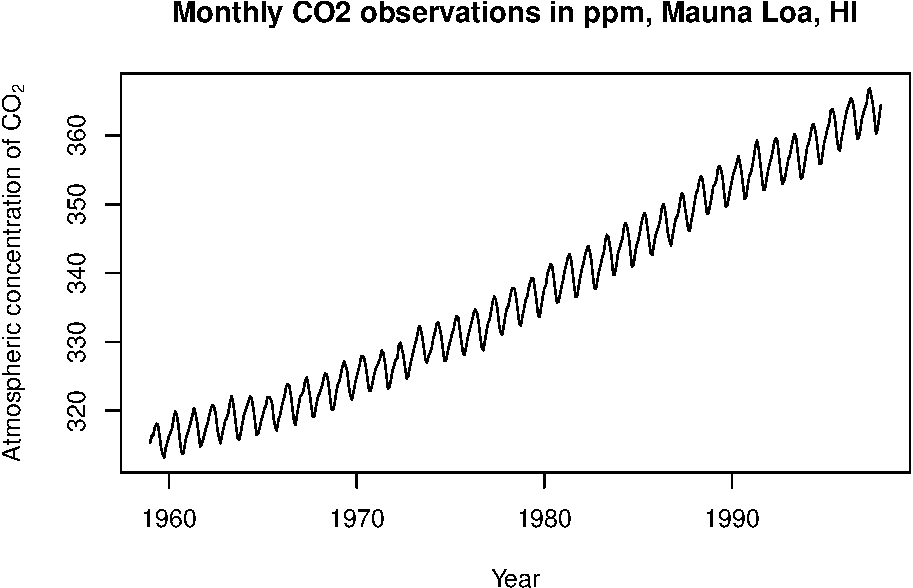
\includegraphics{BIOSCI_0835_files/figure-latex/unnamed-chunk-3-1.pdf}}

\hypertarget{final-exam}{%
\chapter{Final exam}\label{final-exam}}

The final exam will \ldots{}

\begin{enumerate}
\def\labelenumi{\arabic{enumi}.}
\tightlist
\item
  Take place during finals week on the day scheduled by the University
\item
  Be administered in-person using Canvas
\item
  Follow the general format of the unit tests, including having buffer points.
\item
  Potentially improve your grade on another test (see policies elswhere in the syllabus).
\item
  The final exam is NOT one of the 4 unit tests and NOT one of the 3 of those tests that count towards your grade.
\end{enumerate}

Note: I do not hold office hours during finals week.

Questions on the final exam will be of similar difficulty as the regular unit tests.

I can only provide estimated grades prior to the exam.

Information about the final exam schedule for the University can be found here:
\url{https://www.registrar.pitt.edu/students/final-exams}.

What if I have more than one final exam on the same day?
If you have multiple finals scheduled for the same day see here:
\url{https://www.registrar.pitt.edu/sites/default/files/pdf/final_guideline.pdf}

\hypertarget{exam-study-guides}{%
\chapter{Exam study guides}\label{exam-study-guides}}

When lecturing I try to minimize diversions and content that will not be assessed on an exam. In my slides I will flag information as ``background'' or ``not on the test'' when necessary.

In general I don't require you to memorize numbers or dates, and any excepts will be clearly marked in my slides.

I also don't require you to remember the names of people (e.g.~famous scientists) or events in their lives. The only standing exception to this is Charles Darwin - any time I talk about Darwin's life its important. Any other exception will be clearly noted.

In contrast, vocab is very important. Unless stated otherwise all vocab is important and could be on the test.

\hypertarget{study-guides}{%
\section{Study guides}\label{study-guides}}

Given the above, when preparing for the tests the best study guides are:

\begin{enumerate}
\def\labelenumi{\arabic{enumi}.}
\tightlist
\item
  Lecture slides
\item
  Your notes
\end{enumerate}

Exam study guides MAY be made available before each test but these study guides are in no way complete, comprehensive, or representative.

If they are available, I'll let you know.

If available, they are most useful to look over AFTER you have thoroughly reviewed all your other class materials.

\hypertarget{test-grading-policies}{%
\chapter{Test grading policies}\label{test-grading-policies}}

\hypertarget{number-of-tests-dropreplace-policy.}{%
\section{Number of tests \& drop/replace policy.}\label{number-of-tests-dropreplace-policy.}}

\begin{itemize}
\tightlist
\item
  There will be 4 tests administered throughout the semester.
\item
  The final exam will be cumulative.
\item
  No makeup exams will be given for any reason.
\item
  Your lowest scores of the 4 mini-test will be automatically dropped when grades are calculated at the end of the semester.\\
\item
  Additionally, your score on the final can replace your 2nd lowest score, if the final is higher. If your score on the final is lower it does not lower your previous test score.
\item
  Your grade will therefore be based on your 4 best scores plus the final; 1 of those 4 can be modified by the final, so the final can count twice.
\item
  If you are unable to take a unit test for ANY reason it will be counted zero.
\item
  If you miss just 1 test, that score will be automatically dropped as your lowest score when grades are calculated after the final.
\item
  If you miss 2 tests, 1 will be dropped and the 2nd can be replaced by your score on the final.
\item
  If you miss 3 tests, the 3rd zero will remain a zero. If this occurs please contact your advisors to consider your options.
\end{itemize}

\hypertarget{test-length-format}{%
\section{Test length \& format}\label{test-length-format}}

NOTE: the following policies are provisional and may be adjusted as needed to optimize test length and how to implement the ``buffer question'' policy in Canvas.

\begin{itemize}
\tightlist
\item
  Tests will be scored out of 25 points. However, there will be at least 27 points worth of questions on the test. Each test therefore will effectively contain 2 or ``buffer points'' that you can miss without harming your grade.
\item
  The maximum score on a mini-test will always be capped at 25/25. If there are 27 points on a test and you get all 27 questions correct your score will be 100\%.
\item
  No extra credit will be offered on tests; the maximum score on a test will be 100\%.
\end{itemize}

\hypertarget{test-question-formats}{%
\section{Test question formats}\label{test-question-formats}}

\begin{itemize}
\tightlist
\item
  Test questions will frequently be multiple choice. Keyword: ``frequently'' - there will other types of questions too.
\item
  Most tests will have at least one question requiring a numeric calculation.\\
\item
  Other common forms of questions are fill in the blank, dropdowns, or matching.
\item
  There will likely NO True/False questions on tests.
\item
  For fill-in-the-blank questions, spelling errors will result in 0 points. No partial credit will be given.
\end{itemize}

\hypertarget{tests}{%
\chapter{Tests}\label{tests}}

\hypertarget{general-test-policies-information}{%
\section{General Test policies \& Information:}\label{general-test-policies-information}}

\begin{enumerate}
\def\labelenumi{\arabic{enumi}.}
\tightlist
\item
  Tests will be administered in-class but taken on Canvas.
\item
  There will be 4 mini-tests during the semester. 1 will be dropped as detailed elsewhere in the syllabus.
\item
  There are approximately 4.5 weeks of material per test.
\item
  I will not answer questions during the test. This is my normal policy during my other classes, and also is in line with COVID social distancing policies.
\item
  Though I do not currently plan on doing this, I reserve the right to require anyone with an accommodation (e.g.~DRS, quarantine) to take the test remotely to log into Zoom and have your camera on while taking tests.
\end{enumerate}

\hypertarget{testing-technology-policies}{%
\section{Testing technology policies}\label{testing-technology-policies}}

\begin{enumerate}
\def\labelenumi{\arabic{enumi}.}
\tightlist
\item
  If you accidently exit and re-enter the exam you must restart it.
\item
  It is your responsibility to assure that you have adequate power to your device and internet access.
\item
  Devices can be borrowed from the library if necessary.
\item
  If a power or WiFi issue beyond our control impacts the class the test may be re-schedule.
\end{enumerate}

\hypertarget{tophat}{%
\chapter{TopHat}\label{tophat}}

We will use TopHat in-class and for homework. Please bring a charged TopHat compatible device to all lectures and recitations.

\href{www.tophat.com}{\textbf{TopHat}}\\
Join Code: \textbf{907997}\\
www.tophat.com

When logging into TopHat it will ask you for your university. Typing in ``University of Pittsburgh'' brings up 3 options: \textbf{select the first one} that just says ``University of Pittsburgh''.

If this is your first time using TopHat see \href{https://canvas.pitt.edu/courses/106737/pages/joining-tophat?module_item_id=2272350}{Joining TopHat} for more information.

\hypertarget{updates-to-schedule-syllabus}{%
\chapter{Updates to schedule \& syllabus}\label{updates-to-schedule-syllabus}}

I reserve the right to update the syllabus, schedule, point allocation and all other components of the course as necessary.

If changes occur after the first day of class, they will be clearly communicated in class and via email, and a revised syllabus and schedule distributed with major changes flagged.

\hypertarget{videos-of-lectures}{%
\chapter{Videos of lectures}\label{videos-of-lectures}}

The first two weeks of class lecture will be recorded using Zoom and posted to Panopto.

After the first lecture I will distribute the Panopto folder where the videos will be saved.

Note: Since this class is not meant to be taken asynchronously I will not actively support use of these videos.

\hypertarget{zoom}{%
\chapter{Zoom}\label{zoom}}

Class will be in-person and streamed live via Zoom the first two weeks.

\url{https://pitt.zoom.us/j/99372114800}\strut \\
Password: ``BLOSUM''

\end{document}
